\documentclass[11pt]{article}
\usepackage[margin=1in]{geometry}
\usepackage{amsmath}
\usepackage{amssymb}
\usepackage{tikz}
\usetikzlibrary{shapes.geometric, arrows, positioning}
\usepackage{xcolor}
\usepackage{hyperref}

% Define colors for trust levels
\definecolor{trusted}{RGB}{144,238,144}      % Light green
\definecolor{semitrusted}{RGB}{255,165,0}    % Orange
\definecolor{untrusted}{RGB}{255,99,71}      % Tomato red

% Define styles for DFD elements
\tikzstyle{process} = [circle, minimum width=1.5cm, minimum height=1.5cm, text centered, draw=black, fill=trusted, font=\small]
\tikzstyle{entity} = [rectangle, minimum width=2cm, minimum height=1cm, text centered, draw=black, font=\small]
\tikzstyle{datastore} = [rectangle, minimum width=2.5cm, minimum height=0.8cm, text centered, draw=black, double, font=\small]
\tikzstyle{arrow} = [thick,->,>=stealth]

\title{Veri-Store Security Model}
\author{Mac Payton \& Albert Huynh}
\date{February 16, 2026 \\ Version 0.1}

\begin{document}

\maketitle

\tableofcontents
\newpage

\section{Introduction}

% COMMENT: This section provides an overview of the veri-store system and the purpose of this
% security model. Describe the system as a distributed erasure-coded object storage system with
% homomorphic fingerprint verification. State that this is a living document that will evolve as
% the system is developed. Mention that this model follows the threat modeling approach outlined
% by Torr (Microsoft, 2005).

\subsection{Document Purpose}

% COMMENT: Explain that this document serves as the security foundation for the veri-store project.
% It will be used to identify threats, design mitigations, and verify security properties throughout
% the development lifecycle. Note that this is version 0.1 and will be updated as components are
% implemented and new threats are discovered.

\subsection{System Overview}

% COMMENT: Provide a 3-5 sentence high-level description of veri-store: a distributed storage
% system that splits data blocks into fragments using Reed-Solomon erasure coding (m-of-n),
% distributes fragments across multiple servers, and uses homomorphic fingerprints to verify
% fragment integrity without reconstructing the full block. Mention the key security goal:
% ensuring data integrity and authenticity in a potentially adversarial distributed environment.

\section{Scoping}

% COMMENT: Define what is included and excluded from this security model. Specify that this
% model covers the veri-store core system components: fingerprinting, erasure coding, storage,
% verification, and network communication. List what is explicitly out of scope (e.g., operating
% system security, physical server security, user authentication mechanisms). Note that as a
% prototype/academic project, some production concerns may be deferred to future work.

\subsection{In Scope}

% COMMENT: List the specific components and functionality included in this security analysis.
% Examples: homomorphic fingerprint generation and verification, erasure code encoding/decoding,
% fragment storage and retrieval, cross-checksum verification protocol, inter-server communication,
% and data integrity guarantees.

\subsection{Out of Scope}

% COMMENT: List what is explicitly not covered by this security model. Examples: physical security
% of servers, operating system vulnerabilities, DoS attacks on network infrastructure, user
% authentication/authorization (assuming authenticated users), Byzantine fault tolerance beyond
% what homomorphic fingerprints provide. Document these as assumptions or dependencies.

\section{Use Scenarios}

% COMMENT: Describe how veri-store will be deployed and used in practice. Include 3-5 concrete
% deployment scenarios: e.g., local network deployment with 5 storage servers using 3-of-5
% encoding, cloud deployment across multiple availability zones, research/academic usage for
% testing erasure coding systems. Avoid marketing language; focus on operational details relevant
% to security analysis.

\subsection{Primary Use Case}

% COMMENT: Describe the main expected usage: a client application storing data blocks across
% multiple servers in a local network or cloud environment. Specify that clients can store,
% retrieve, and verify data integrity. Note whether this is single-user or multi-user, whether
% servers are trusted or semi-trusted, and what network environment is assumed (LAN vs Internet).

\subsection{Anti-Scenarios}

% COMMENT: List configurations or usage patterns that are explicitly unsupported or known to be
% insecure. Examples: running storage servers on untrusted/compromised machines, using veri-store
% for real-time/low-latency applications, storing unencrypted sensitive data (if encryption is
% out of scope), relying on veri-store for availability guarantees beyond erasure coding provides.

\section{Dependencies}

% COMMENT: Enumerate all external libraries, systems, and services that veri-store relies upon.
% For each dependency, note what functionality it provides and what security assumptions you're
% making about it. Examples: Python standard library, galois/pyfinite for finite field arithmetic,
% numpy for array operations, network stack (TCP/IP), file system for local storage.

\subsection{External Libraries}

\begin{itemize}
\item \textbf{galois}: % Finite field arithmetic over F_256
\item \textbf{numpy}: % Array operations and polynomial manipulation
\item \textbf{Python standard library}: % Networking, file I/O, cryptographic primitives
\end{itemize}

\subsection{System Dependencies}

\begin{itemize}
\item \textbf{Network stack}: % TCP/IP for inter-server communication
\item \textbf{File system}: % Local storage of fragments
\item \textbf{Operating system}: % Process isolation, memory protection
\end{itemize}

\section{Implementation Assumptions}

% COMMENT: List all assumptions made during design and development that must be verified later.
% These help scope the threat model and identify areas where assumptions might be invalid.
% Examples: servers do not collude beyond f failures, network provides reliable delivery,
% cryptographic primitives (if used) are secure, finite field arithmetic is correctly implemented,
% fragment storage is atomic.

\begin{itemize}
\item placeholder % At most f out of n servers may be compromised or fail
\item placeholder % Network communication channels are authenticated (or will be)
\item placeholder % Storage servers have sufficient disk space for fragments
\item placeholder % Homomorphic fingerprint collision probability is negligible
\item placeholder % Erasure coding library correctly implements Reed-Solomon
\end{itemize}

\section{Trust Levels}

% COMMENT: Define the hierarchy of trust levels in the system. For each trust level, describe
% what entities operate at that level and what capabilities/privileges they have. In distributed
% systems, this often includes: system administrator, authenticated client, storage server,
% untrusted network attacker. Note that some components may operate at different trust levels
% depending on deployment scenario.

\subsection{Administrator}

% COMMENT: Describe the system administrator trust level. This includes anyone with physical or
% root access to the servers. Administrators have complete control over the system and can read,
% modify, or delete any data. Security model assumes administrators are trusted and benign.

\subsection{Authenticated Client}

% COMMENT: Describe clients who have authenticated to the system and are authorized to store/retrieve
% data. These users are assumed to be legitimate but may make mistakes or run buggy software.
% They should not be able to corrupt other users' data or violate system integrity.

\subsection{Storage Server}

% COMMENT: Describe the trust level of storage servers. In the semi-trusted model, servers might
% fail, return corrupted data, or attempt to forge fingerprints, but do not actively collude
% (beyond the f-threshold). Specify whether servers are assumed to follow protocols correctly or
% might exhibit Byzantine behavior.

\subsection{Untrusted Network}

% COMMENT: Describe the untrusted network attacker model. This includes any adversary who can
% observe, modify, or inject network traffic between clients and servers or between servers.
% Network attackers cannot compromise server storage but can manipulate messages in transit.
% Specify whether you assume network authentication (TLS) or if that's future work.

\section{Entry Points}

% COMMENT: List all interfaces where external entities interact with veri-store. Each entry point
% represents a potential attack surface. Group related operations into logical categories rather
% than listing every API method. For each entry point, note its trust level and whether it sends
% or receives data (or both). Examples: client API for store/retrieve, inter-server verification
% protocol, storage subsystem file operations.

\subsection{Client API}

\begin{itemize}
\item \textbf{Store operation}: % Client submits data block for encoding and distribution
\item \textbf{Retrieve operation}: % Client requests data block reconstruction from fragments
\item \textbf{Verify operation}: % Client checks data integrity using fingerprints
\end{itemize}

\subsection{Inter-Server Communication}

\begin{itemize}
\item \textbf{Fingerprint exchange}: % Servers share fingerprints for cross-checksum verification
\item \textbf{Fragment retrieval}: % Servers request fragments from peers for reconstruction
\end{itemize}

\subsection{Storage Subsystem}

\begin{itemize}
\item \textbf{Fragment write}: % Store encoded fragment to local disk
\item \textbf{Fragment read}: % Retrieve fragment from local disk
\item \textbf{Fingerprint storage}: % Store/retrieve homomorphic fingerprints
\end{itemize}

\section{Protected Assets}

% COMMENT: Identify all resources that must be protected from harm. These are the things an
% attacker will try to steal, modify, or disrupt. For each asset, specify what trust levels
% should have access to it and what properties must be maintained (confidentiality, integrity,
% availability). Examples: original data blocks, erasure-coded fragments, homomorphic fingerprints,
% cryptographic keys (if used), server resources (CPU, memory, disk).

\subsection{Data Blocks}

% COMMENT: Original data blocks submitted by clients. Primary security concern is integrity:
% ensuring retrieved data matches what was stored. Confidentiality may be out of scope if
% encryption is handled separately. Availability depends on having at least m of n fragments
% available.

\subsection{Erasure-Coded Fragments}

% COMMENT: Individual fragments stored on servers. Must maintain integrity to ensure correct
% reconstruction. Fragment authenticity is verified via homomorphic fingerprints. Loss of fewer
% than n-m fragments should not compromise data availability.

\subsection{Homomorphic Fingerprints}

% COMMENT: Compact cryptographic checksums that preserve erasure code structure. Critical for
% integrity verification. Must be protected from tampering and forgery. Fingerprints themselves
% don't reveal data content but must be authentic.

\subsection{System Resources}

% COMMENT: Server computational resources (CPU, memory, disk space, network bandwidth). Attackers
% should not be able to exhaust these resources and cause denial of service. Resource consumption
% should be proportional to legitimate usage.

\section{Data Flow Diagram}

% COMMENT: This section contains the graphical representation of data flows through veri-store.
% The DFD shows all major components, entry points, data stores, and how information moves
% between them. Use different colors for trust levels: green for trusted processes, red for
% untrusted entities/data, orange for semi-trusted. Number all data flows sequentially and label
% them with concise descriptions.

\begin{figure}[ht!]
\centering
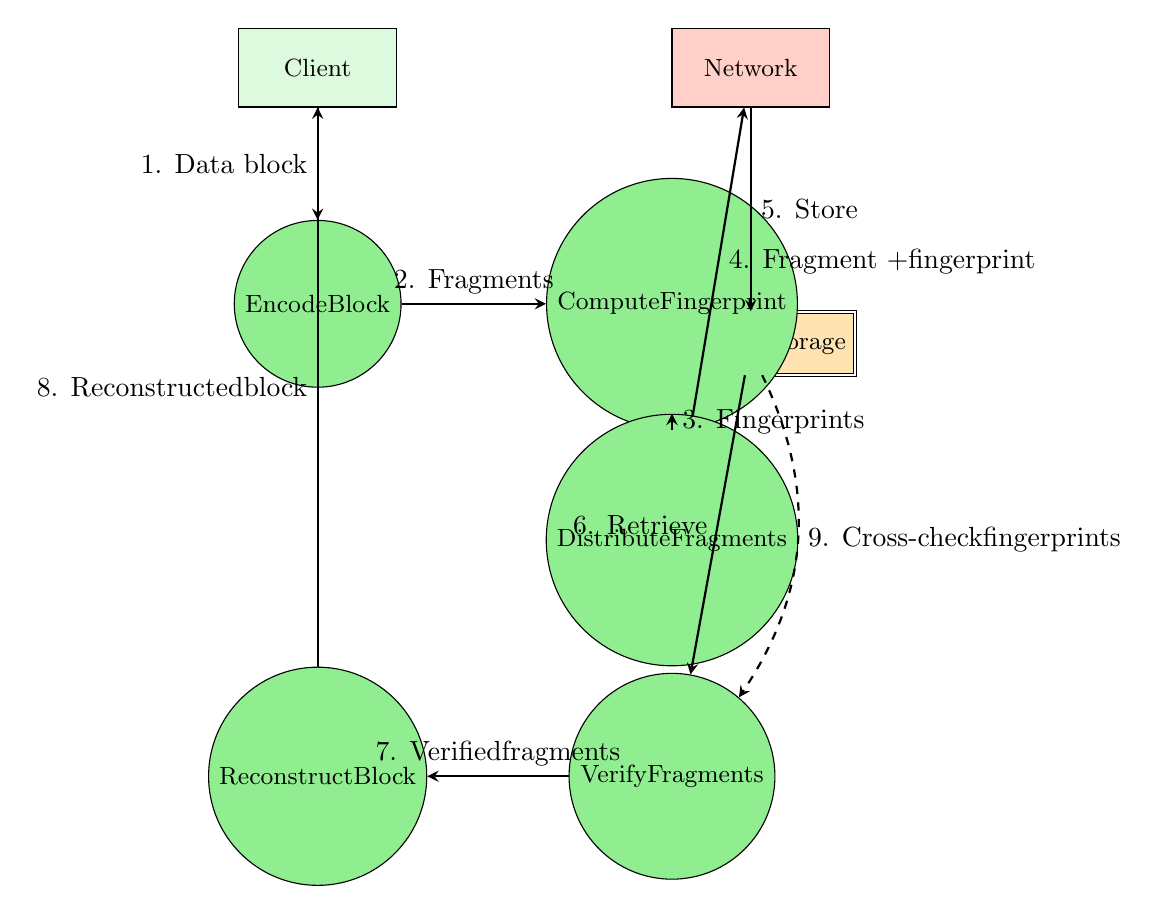
\begin{tikzpicture}[node distance=2.5cm]

% External entities
\node (client) [entity, fill=trusted!30] {Client};
\node (network) [entity, fill=untrusted!30, right of=client, xshift=3cm] {Network};
\node (storage) [datastore, fill=semitrusted!30, below of=network, yshift=-1cm] {Fragment \newline Storage};

% Processes (all trusted - our code)
\node (encode) [process, below of=client, yshift=-0.5cm] {Encode \newline Block};
\node (fingerprint) [process, right of=encode, xshift=2cm] {Compute \newline Fingerprint};
\node (distribute) [process, below of=fingerprint, yshift=-0.5cm] {Distribute \newline Fragments};
\node (verify) [process, below of=distribute, yshift=-0.5cm] {Verify \newline Fragments};
\node (reconstruct) [process, left of=verify, xshift=-2cm] {Reconstruct \newline Block};

% Data flows
\draw [arrow] (client) -- node[anchor=east] {1. Data block} (encode);
\draw [arrow] (encode) -- node[anchor=south] {2. Fragments} (fingerprint);
\draw [arrow] (fingerprint) -- node[anchor=west] {3. Fingerprints} (distribute);
\draw [arrow] (distribute) -- node[anchor=west] {4. Fragment + \newline fingerprint} (network);
\draw [arrow] (network) -- node[anchor=west] {5. Store} (storage);
\draw [arrow] (storage) -- node[anchor=east] {6. Retrieve} (verify);
\draw [arrow] (verify) -- node[anchor=south] {7. Verified \newline fragments} (reconstruct);
\draw [arrow] (reconstruct) -- node[anchor=east] {8. Reconstructed \newline block} (client);

% Cross-checksum verification (dotted line to show verification flow)
\draw [arrow, dashed] (storage) to[bend left=30] node[anchor=west] {9. Cross-check \newline fingerprints} (verify);

\end{tikzpicture}
\caption{High-level data flow diagram for veri-store store and retrieve operations.}
\label{fig:dfd}
\end{figure}

\subsection{DFD Component Descriptions}

% COMMENT: Provide brief descriptions of each component in the DFD. Explain what each process
% does, what trust level it operates at, and what security properties it maintains. Describe
% external entities and data stores. Note any assumptions about data flows (e.g., authenticated
% channels, encrypted storage).

\subsubsection{Client}

% COMMENT: External entity representing the user or application storing/retrieving data. Operates
% at "authenticated client" trust level. Assumed to be benign but may have bugs.

\subsubsection{Encode Block}

% COMMENT: Trusted process that implements Reed-Solomon erasure coding. Takes original block,
% produces n fragments such that any m can reconstruct the original. Must correctly implement
% the encoding algorithm to ensure fragments are valid.

\subsubsection{Compute Fingerprint}

% COMMENT: Trusted process that generates homomorphic fingerprints for each fragment using division
% fingerprinting over F_256. Must use cryptographically secure random parameter r and correctly
% compute fingerprints to ensure collision resistance.

\subsubsection{Distribute Fragments}

% COMMENT: Trusted process that sends fragments and fingerprints to storage servers. Handles
% network communication and retries. May need to authenticate servers to prevent MITM attacks.

\subsubsection{Network}

% COMMENT: Untrusted external entity representing network infrastructure. Adversary may observe,
% modify, or inject messages. Protection via authentication (TLS) or message authentication codes
% may be needed.

\subsubsection{Fragment Storage}

% COMMENT: Semi-trusted data store representing persistent storage on servers. Stores fragments
% and fingerprints. Servers may fail or return corrupted data but are detected via verification.
% Storage is assumed to be persistent but not necessarily confidential.

\subsubsection{Verify Fragments}

% COMMENT: Trusted process that validates fragment integrity using homomorphic fingerprints.
% Retrieves fragments and fingerprints from storage, performs cross-checksum verification to
% detect corrupted or forged fragments. Rejects invalid fragments.

\subsubsection{Reconstruct Block}

% COMMENT: Trusted process that decodes original block from m valid fragments using Reed-Solomon
% decoding. Only operates on verified fragments to ensure integrity of reconstructed data.

\section{Threat Analysis: STRIDE}

% COMMENT: This section applies the STRIDE framework to systematically identify threats. For each
% STRIDE category, list potential threats discovered during brainstorming. Express threats as
% "Entity X performs action Y resulting in negative outcome Z". Don't worry about mitigations yet;
% just document all potential threats. Each threat will be resolved in the next section.

\subsection{Spoofing}

% COMMENT: Threats where attackers pretend to be someone or something else. Examples: impersonating
% legitimate clients, forging server identities, replaying old authentication tokens, masquerading
% as storage servers to receive fragments. Consider both client-to-server and server-to-server
% authentication.

\subsubsection{S.1: Client Impersonation}

% THREAT: An attacker impersonates a legitimate client and stores malicious data or retrieves
% other users' data.

\subsubsection{S.2: Server Impersonation}

% THREAT: An attacker impersonates a storage server and receives fragments from clients, potentially
% learning information about stored data.

\subsubsection{S.3: Fingerprint Source Forgery}

% THREAT: An attacker forges the source of fingerprints during cross-checksum verification,
% causing servers to trust malicious fingerprint values.

\subsection{Tampering}

% COMMENT: Threats where attackers modify data in transit or at rest. Examples: corrupting
% fragments in storage, modifying fragments in transit, tampering with fingerprints, altering
% encoded data before distribution. Consider both accidental corruption and malicious modification.

\subsubsection{T.1: Fragment Corruption in Storage}

% THREAT: A malicious or compromised storage server modifies fragments at rest, causing data
% corruption that will be detected only upon retrieval.

\subsubsection{T.2: Fragment Modification in Transit}

% THREAT: A network attacker intercepts and modifies fragments or fingerprints during transmission
% between client and servers or between servers.

\subsubsection{T.3: Fingerprint Tampering}

% THREAT: An attacker modifies fingerprints to match corrupted fragments, bypassing integrity
% verification.

\subsubsection{T.4: Erasure Code Parameter Manipulation}

% THREAT: An attacker manipulates encoding parameters (m, n, or field size) causing incorrect
% encoding that appears valid but cannot be decoded.

\subsection{Repudiation}

% COMMENT: Threats where attackers perform actions that cannot be traced back to them. Examples:
% storing data without audit trail, deleting fragments without logging, modifying data with no
% accountability. This may be less critical for an academic prototype but should be considered
% for production systems.

\subsubsection{R.1: Anonymous Data Storage}

% THREAT: An attacker stores large amounts of data without accountability, potentially consuming
% storage resources or storing illegal content.

\subsubsection{R.2: Fragment Deletion Without Logging}

% THREAT: A compromised server deletes fragments without creating audit records, making it
% impossible to trace data loss to specific servers.

\subsubsection{R.3: Untrackable Verification Failures}

% THREAT: When verification fails, the system cannot determine which server provided corrupted
% data, allowing malicious servers to evade detection.

\subsection{Information Disclosure}

% COMMENT: Threats where attackers steal or learn sensitive information. Examples: reading
% fragments from storage, inferring data patterns from fingerprints, eavesdropping on network
% traffic, exploiting verbose error messages. Consider whether data confidentiality is in scope
% or if encryption is assumed to be handled separately.

\subsubsection{I.1: Fragment Eavesdropping}

% THREAT: A network attacker intercepts fragments in transit and reconstructs the original block
% if they capture at least m fragments.

\subsubsection{I.2: Storage Server Data Access}

% THREAT: A compromised storage server reads all fragments it stores, potentially learning
% partial information about data blocks.

\subsubsection{I.3: Fingerprint Analysis}

% THREAT: An attacker analyzes fingerprints to infer information about data content, though
% fingerprints are designed to reveal minimal information.

\subsubsection{I.4: Error Message Information Leakage}

% THREAT: Verbose error messages reveal internal system state, cryptographic parameters, or
% fragment locations that could aid attacks.

\subsection{Denial of Service}

% COMMENT: Threats where attackers disrupt legitimate system operation. Examples: exhausting
% storage capacity, flooding network with requests, corrupting fragments to make data unrecoverable,
% causing expensive cryptographic operations. Consider both resource exhaustion and functional
% denial of service.

\subsubsection{D.1: Storage Exhaustion}

% THREAT: An attacker stores excessive data, filling storage servers and preventing legitimate
% users from storing data.

\subsubsection{D.2: Fragment Unavailability}

% THREAT: An attacker compromises more than n-m servers or corrupts more than n-m fragments,
% making data unrecoverable.

\subsubsection{D.3: Verification Flooding}

% THREAT: An attacker triggers excessive verification operations, consuming CPU resources with
% expensive finite field arithmetic and cryptographic operations.

\subsubsection{D.4: Network Bandwidth Exhaustion}

% THREAT: An attacker floods the network with fragment requests or verification messages,
% preventing legitimate communication.

\subsection{Elevation of Privilege}

% COMMENT: Threats where attackers gain capabilities they are not authorized to have. Examples:
% exploiting buffer overflows to execute arbitrary code, bypassing access controls, escalating
% from client to server privileges. Consider both implementation vulnerabilities and design flaws.

\subsubsection{E.1: Code Injection via Malformed Input}

% THREAT: An attacker sends maliciously crafted fragments or fingerprints that exploit parsing
% vulnerabilities, leading to arbitrary code execution on servers.

\subsubsection{E.2: Verification Bypass}

% THREAT: An attacker discovers a way to bypass fingerprint verification, allowing corrupted
% fragments to be accepted as valid.

\subsubsection{E.3: Cryptographic Parameter Override}

% THREAT: An attacker manipulates system parameters (fingerprint size, field size, collision
% probability) to weaken security and enable attacks.

\subsubsection{E.4: Server-to-Server Privilege Escalation}

% THREAT: A compromised storage server exploits inter-server protocols to gain control over
% other servers or access fragments it should not have.

\section{Threat Resolutions}

% COMMENT: For each threat identified in the previous section, document its resolution. Classify
% each threat as: (1) already mitigated by current design, (2) mitigated by dependency,
% (3) requires mitigation, (4) dependency's responsibility, or (5) accepted risk. For mitigated
% threats, describe the mitigation and assign testing to verify it. For unmitigated threats
% requiring action, assign an owner and track to completion.

\subsection{Spoofing Threat Resolutions}

\subsubsection{S.1: Client Impersonation}
\begin{itemize}
\item \textbf{Status}: % Requires mitigation / Dependency responsibility / Accepted risk
\item \textbf{Resolution}: % Description of how this threat will be addressed
\item \textbf{Owner}: % Person responsible for implementation/verification
\item \textbf{Testing}: % How this mitigation will be verified
\end{itemize}

\subsubsection{S.2: Server Impersonation}
\begin{itemize}
\item \textbf{Status}: %
\item \textbf{Resolution}: %
\item \textbf{Owner}: %
\item \textbf{Testing}: %
\end{itemize}

\subsubsection{S.3: Fingerprint Source Forgery}
\begin{itemize}
\item \textbf{Status}: %
\item \textbf{Resolution}: %
\item \textbf{Owner}: %
\item \textbf{Testing}: %
\end{itemize}

\subsection{Tampering Threat Resolutions}

\subsubsection{T.1: Fragment Corruption in Storage}
\begin{itemize}
\item \textbf{Status}: % Already mitigated by homomorphic fingerprint verification
\item \textbf{Resolution}: % Cross-checksum protocol detects corrupted fragments
\item \textbf{Owner}: %
\item \textbf{Testing}: % Test suite injects corrupted fragments and verifies detection
\end{itemize}

\subsubsection{T.2: Fragment Modification in Transit}
\begin{itemize}
\item \textbf{Status}: %
\item \textbf{Resolution}: %
\item \textbf{Owner}: %
\item \textbf{Testing}: %
\end{itemize}

\subsubsection{T.3: Fingerprint Tampering}
\begin{itemize}
\item \textbf{Status}: %
\item \textbf{Resolution}: %
\item \textbf{Owner}: %
\item \textbf{Testing}: %
\end{itemize}

\subsubsection{T.4: Erasure Code Parameter Manipulation}
\begin{itemize}
\item \textbf{Status}: %
\item \textbf{Resolution}: %
\item \textbf{Owner}: %
\item \textbf{Testing}: %
\end{itemize}

\subsection{Repudiation Threat Resolutions}

\subsubsection{R.1: Anonymous Data Storage}
\begin{itemize}
\item \textbf{Status}: %
\item \textbf{Resolution}: %
\item \textbf{Owner}: %
\item \textbf{Testing}: %
\end{itemize}

\subsubsection{R.2: Fragment Deletion Without Logging}
\begin{itemize}
\item \textbf{Status}: %
\item \textbf{Resolution}: %
\item \textbf{Owner}: %
\item \textbf{Testing}: %
\end{itemize}

\subsubsection{R.3: Untrackable Verification Failures}
\begin{itemize}
\item \textbf{Status}: %
\item \textbf{Resolution}: %
\item \textbf{Owner}: %
\item \textbf{Testing}: %
\end{itemize}

\subsection{Information Disclosure Threat Resolutions}

\subsubsection{I.1: Fragment Eavesdropping}
\begin{itemize}
\item \textbf{Status}: %
\item \textbf{Resolution}: %
\item \textbf{Owner}: %
\item \textbf{Testing}: %
\end{itemize}

\subsubsection{I.2: Storage Server Data Access}
\begin{itemize}
\item \textbf{Status}: %
\item \textbf{Resolution}: %
\item \textbf{Owner}: %
\item \textbf{Testing}: %
\end{itemize}

\subsubsection{I.3: Fingerprint Analysis}
\begin{itemize}
\item \textbf{Status}: %
\item \textbf{Resolution}: %
\item \textbf{Owner}: %
\item \textbf{Testing}: %
\end{itemize}

\subsubsection{I.4: Error Message Information Leakage}
\begin{itemize}
\item \textbf{Status}: %
\item \textbf{Resolution}: %
\item \textbf{Owner}: %
\item \textbf{Testing}: %
\end{itemize}

\subsection{Denial of Service Threat Resolutions}

\subsubsection{D.1: Storage Exhaustion}
\begin{itemize}
\item \textbf{Status}: %
\item \textbf{Resolution}: %
\item \textbf{Owner}: %
\item \textbf{Testing}: %
\end{itemize}

\subsubsection{D.2: Fragment Unavailability}
\begin{itemize}
\item \textbf{Status}: %
\item \textbf{Resolution}: %
\item \textbf{Owner}: %
\item \textbf{Testing}: %
\end{itemize}

\subsubsection{D.3: Verification Flooding}
\begin{itemize}
\item \textbf{Status}: %
\item \textbf{Resolution}: %
\item \textbf{Owner}: %
\item \textbf{Testing}: %
\end{itemize}

\subsubsection{D.4: Network Bandwidth Exhaustion}
\begin{itemize}
\item \textbf{Status}: %
\item \textbf{Resolution}: %
\item \textbf{Owner}: %
\item \textbf{Testing}: %
\end{itemize}

\subsection{Elevation of Privilege Threat Resolutions}

\subsubsection{E.1: Code Injection via Malformed Input}
\begin{itemize}
\item \textbf{Status}: %
\item \textbf{Resolution}: %
\item \textbf{Owner}: %
\item \textbf{Testing}: %
\end{itemize}

\subsubsection{E.2: Verification Bypass}
\begin{itemize}
\item \textbf{Status}: %
\item \textbf{Resolution}: %
\item \textbf{Owner}: %
\item \textbf{Testing}: %
\end{itemize}

\subsubsection{E.3: Cryptographic Parameter Override}
\begin{itemize}
\item \textbf{Status}: %
\item \textbf{Resolution}: %
\item \textbf{Owner}: %
\item \textbf{Testing}: %
\end{itemize}

\subsubsection{E.4: Server-to-Server Privilege Escalation}
\begin{itemize}
\item \textbf{Status}: %
\item \textbf{Resolution}: %
\item \textbf{Owner}: %
\item \textbf{Testing}: %
\end{itemize}

\section{External Security Notes}

% COMMENT: Document any security-relevant information that should be communicated to users,
% deployers, or other teams. This includes known limitations, security best practices for
% deployment, configuration recommendations, and any threats that are out of scope for veri-store
% but users should be aware of. Examples: recommend using TLS for network communication,
% suggest server isolation strategies, note that data confidentiality requires client-side encryption.

\subsection{Deployment Recommendations}

% COMMENT: Provide guidance on secure deployment of veri-store. What network configurations are
% recommended? Should servers be isolated? What authentication mechanisms should be used?

\subsection{Known Limitations}

% COMMENT: Document security limitations that users should be aware of. What attacks does the
% system NOT protect against? What trust assumptions are made? Under what conditions might
% security guarantees not hold?

\subsection{Integration Considerations}

% COMMENT: If veri-store is used as a component in a larger system, what security properties
% does it provide and what must be handled by the integrating system? For example: veri-store
% ensures integrity but not confidentiality; authentication must be provided by the application.

\section{Verification and Testing Plan}

% COMMENT: Outline how you will verify that security mitigations are implemented correctly and
% continue to work as the system evolves. This includes unit tests for security-critical code,
% integration tests for security protocols, penetration testing, code review process, and
% regression testing. Specify who is responsible for creating and maintaining security tests.

\subsection{Security Test Suite}

% COMMENT: Describe the automated test suite that will verify security properties. Tests should
% cover: fingerprint collision resistance, detection of corrupted fragments, verification protocol
% correctness, proper handling of malformed input. Each mitigated threat should have corresponding
% tests.

\subsection{Code Review Process}

% COMMENT: Define the code review process for security-critical components. What criteria must
% be met? Who performs reviews? Are there specific areas (fingerprinting, network protocol) that
% require extra scrutiny?

\subsection{Regression Testing}

% COMMENT: Explain how you will prevent security regressions as the code evolves. Security tests
% must be run on every commit. Design changes must trigger threat model review to ensure
% assumptions remain valid.

\section{Document Maintenance}

% COMMENT: Establish procedures for keeping this security model up-to-date. Specify when the
% document should be reviewed and updated: after major design changes, when new components are
% added, at project milestones, before releases. Assign responsibility for maintaining the document.

\subsection{Review Schedule}

% COMMENT: Define when this document will be reviewed. Examples: weekly during active development,
% at the end of each project milestone, when dependencies are updated, before any demo or
% presentation to external stakeholders.

\subsection{Change Process}

% COMMENT: Describe the process for updating this document. Who can make changes? What triggers
% an update? How are changes communicated to the team? Ensure all stakeholders are notified
% when security assumptions or threat resolutions change.

\subsection{Version History}

\begin{itemize}
\item \textbf{Version 0.1} (February 16, 2026): Initial draft - high-level security model with component stubs
\end{itemize}

\end{document}
